\documentclass[11pt,a4paper]{article}

\usepackage[utf8]{inputenc}
\usepackage{siunitx}
\usepackage{geometry}
\newgeometry{margin=2.0cm}

\usepackage[backend=biber,style=authoryear,sorting=nyt,dashed=false]{biblatex}
\renewcommand*{\nameyeardelim}{\addcomma\space}
\addbibresource{references/references.bib} % note the .bib is required

\newcommand*\mean[1]{\overline{#1}}

\title{Effects of Vertical Shear on Cloud Field Variability and Organization }
\author{Mark Muetzelfeldt}
\date{April 2017}

\begin{document}

\maketitle

\subsection*{Main papers (*:key papers)}
\begin{itemize}
    \item * \cite{CC2006I}
    \item * \cite{CC2006II}
    \item * \cite{RE2001}
    \item * \cite{RKW1988}
    \item * \cite{PC2008}
    \item \cite{birch2014scale}
    \item \cite{cohen2004response}
    \item \cite{gregory1997parametrization}
    \item \cite{houze1977structure}
    \item \cite{kershaw1997parametrization}
    %\item \cite{parker2007simulated}
    \item \cite{robe1996moist}
    \item \cite{sakradzija2016stochastic}
    \item \cite{sengupta1990cumulus}
    \item \cite{TMM1982}
\end{itemize}

\section{Introduction}

%\begin{itemize}
%    \item Justification for using RCE - links to QE.
%    \item Motivation for how this work fits into larger picture of stochastic parametrization. Particularly the variability analysis.
%    \item Set out experimental design: choice of shear profiles and explanation of why these produce organization, linking back to previous work, e.g. \cite{RKW1988}.
%    \item Mention: organization and momentum flux.
%\end{itemize}

Most moist convection parametrization schemes in use are deterministic - for a given grid-column state they will produce a single specific amount of convective heating, moistening and perhaps momentum transport. This can be justified through the Quasi-Equilibrium (QE) assumption of \cite{arakawa1974}, in which it is assumed that the convection is in local equilibrium with the grid-scale forcing because each grid-column contains many convective plumes. As model resolution increases, this assumption will breakdown, as each grid-column contains fewer and fewer convective plumes. One way of modelling the parametrized convection in these circumstances is by using a stochastic parametrization scheme - the magnitude of the subgrid convection is not determined by sampling from a Probability Distribution Function (PDF) instead of being uniquely determined by the grid-scale state.

Stochastic parametrization schemes require a characterization of the subgrid variability of the convection. This can be done by using Cloud Resolving Models (CRMs) to verify the theoretical models of how the variability of the convection is distributed. In this study, we look at how the organization of deep convection affects the variability of the convection. In particular, we look at how squall lines consisting generated by deep vertical shear in the troposphere modify the distribution of convective mass flux.

CRMs can exhibit different modes of organization. For example, when run with interactive radiation, CRMs can display self-aggregation. This is where convection develops in a large subregion of the domain, often related to the scale of the model, whilst outside of this region compensating subsidence occurs. The mechanisms for this are disputed, and may be different from model to model. However, interactive radiation, or a prescribed cooling profile that varies across the domain, is necssary. As we with to isolate the organization stimulated by shear, we use a uniform prescribed cooling profile over our domain. This also means we can effectively vary the amount of convection by increasing the magnitude of the cooling.

The simulations carried out are run to statistical equilibrium, in the sense that the model state taken over a large enough domain and time period is statistically indistinguishable from another such period. Thus the model as a whole is [representative?] of the QE assumption. However, at smaller spatial or temporal scales, there will be significant departures from this mean state. It is precisely these fluctuations, and their relative frequencies, that we wish to characterize.

The way we charaterize the fluctuations is by investigating the distribution of convective mass flux. Mass flux is a key parameter in convection parametrization schemes, as it value is used to determine the behaviour of a cloud model. This will typically lead to a moistening of the upper troposphere through detrainment from the cloud, as well as a heating of the troposphere, primarily through the compensating subsidence. The magnitude of the mass flux is determined through the use of a closure based on the grid-column state of the model. A popular choice of closure is the Convective Available Potential Energy (CAPE) closure assumption, whereby a percentage of the CAPE is assumed to [be consumed] by the convection in a given timestep. This can be used to set the mass flux by iterating towards the required value or by theoretical arguments. The magnitude of the mass flux then determines how much heating and moistening of the atmosphere will happen because of the unresolved convection, through the use of a cloud model.

\section{Model and experimental design}

\subsection{Model setup}

\begin{itemize}
    \item Using an idealized version of the Met Office Unified Model (version 10.7).
    \item 2 spatial resolutions used: \SI{1}{km} and \SI{2500}{m}. The first allows easier comparison between this and previous studies, the second is better able to capture convection. Running with $\Delta t$ of \SI{30}{s} and \SI{10}{s} respectively.
    \item Running over a domain of 256$\times$256 \SI{}{km^2}, for a duration of \SI{20}{days}. This should be large enough to cover the spatial extent of the squall lines, and long enough to both reach equilibrium and provide a long enough time to average over many squall lines' lifetimes.
    \item Forced with prescribed cooling of \SI{4}{K.day^{-1}} (Or higher?) - typical of radiative cooling rates over the tropics + LS convergence.
    \item Using a 3D Smagorinsky Turbulence scheme, no convection scheme. Includes the OCF MC scheme.
    \item Applying a relaxation back to a neutral profile above \SI{12.5}{km} (or \SI{15}{km}?).
\end{itemize}

\subsection{Shear profiles}

\begin{itemize}
    \item Profiles are applied by relaxing back to a mean wind across the domain.
    \item This takes the form of applying an increment of $u_{inc} = \frac{U_{ref} - <u>}{\tau} \Delta t$. $\tau = $ \SI{21600}{s}.
    \item The momentum flux, can be calculated using $\rho \mean{u' v'} = \rho \frac{u_{inc}}{\Delta t} \Delta z$.
\end{itemize}

\begin{figure}[htp!]
    \centering
    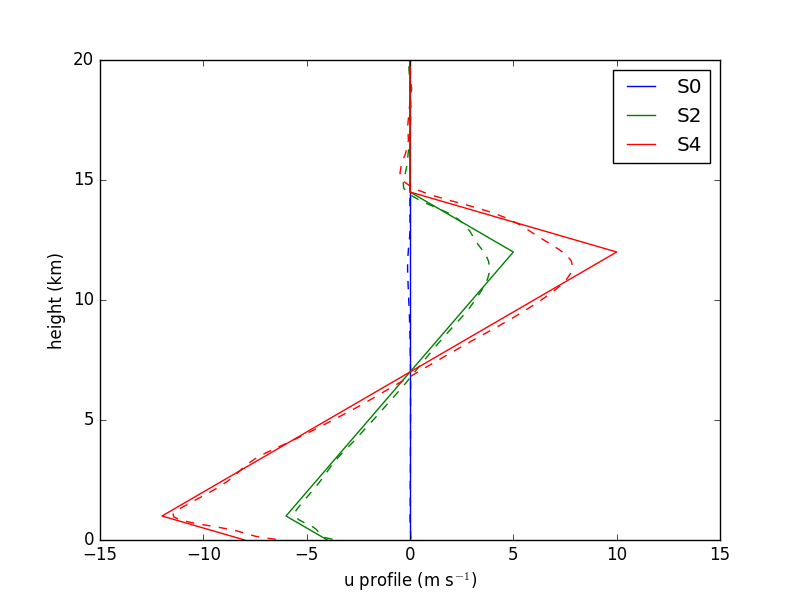
\includegraphics[width=450px]{figs/profile_plot.uv_profile}
    \caption{...}
    \label{fig:MC_on_off}
\end{figure}

\section{Results}
\begin{itemize}
   \item Table 1: List of experiments, S0, S5 etc. plus explanation of each one.

   \item Figure 1: Two snapshots from S0/S5, with no organization and organization present. Something like $w$ at \SI{2500}{m}.
\end{itemize}

\subsection{Spatial variability}
\begin{itemize}
    \item Figure 2: Effects of spatial lengths on total mass-flux (c.f. \cite{PC2008}, Fig. 1).
    \item Figure 3: Effects of spatial lengths on PDF of mass-flux per cloud cell (c.f. \cite{CC2006II}, Fig. 2).
    \item N.B. perhaps combined into one figure.
\end{itemize}

\subsection{Cloud field organization}
\begin{itemize}
    \item Figure 4: Measure of organization demonstrating effectively the higher organization in the organized convection cases.
\end{itemize}

\subsection{Equilibrium profiles}
\begin{itemize}
    \item (Will this be kept?) Figure 5: Difference in equilibrium states from the different experiments. 
\end{itemize}

\subsection{Momentum transports}
\begin{itemize}
    \item Figure 6: Momentum flux profiles for different experiments (c.f. \cite{RE2001}, Fig. 7).
\end{itemize}
\section{Conclusions}

\newpage
\printbibliography[title={References}]


\end{document}
